\documentclass[a4paper,12pt,oneside]{report}
\usepackage[left=2.5cm,right=2.5cm,top=2cm,bottom=3cm]{geometry}
% Created by Yue Li, June 2017
% Adapted by George McCarron, December 2019

\pagestyle{empty}

\setlength{\parskip}{1em}
\setlength{\parindent}{0em}

\makeatletter  %to avoid error messages generated by "\@". Makes Latex treat "@" like a letter

\linespread{1.5}
\def\submitdate#1{\gdef\@submitdate{#1}}
\def\degree#1{\gdef\@degree{#1}}
\def\studentid#1{\gdef\@studentid{#1}}
\def\supervisor#1{\gdef\@supervisor{#1}}

\def\maketitle{
  \begin{center}
    
    
  \includegraphics[width=0.5\columnwidth]{images/nottingham-logo.png} \par
  
  \vskip 1in \par 
  \Huge {\bf 4302306}

  \vskip 0.3in \par
  %\large {\bf \@author} \par
  \large {\bf Supervisor: Prof. Derek McAuley}
  
  \vskip 0.3in \par
  \large {\bf Module Code: G53IDS}

  \vskip 4in \par
  \large {\bf 2020/05}
\end{center}
    
  \begin{titlepage}{
    
    \centering{
    \includegraphics[width=0.5\columnwidth]{images/nottingham-logo.png}} \par
    
    \vskip 1in \par 
    \LARGE {\bf \@title}
  }
  \vskip 0.3in \par
  %\large {\bf \@author} \par
  \large {\bf \@studentid}
  
  \vskip 0.3in \par
  \large {\bf Supervised by \@supervisor}
  \vskip 0.3in \par
  \normalsize { School of Computer Science \par
  University of Nottingham}
  \vskip 0.3in \par
  \normalsize { \@submitdate }

  \vskip 0.5in \par
  \normalsize {Submitted in partial fulfillment of \\ the conditions for the award of the degree \bf{\@degree}.}
  \vskip 0.3in \par
  \normalsize {I hereby declare that this dissertation is all my own work, except as indicated in the text: }

  \vskip 0.5in 
  \normalsize {Signature \underline{\hspace{1.5in}}}
  
  \vskip 0.1in
  \normalsize {Date \underline{\hspace{0.5in}} / \underline{\hspace{0.5in}} / \underline{\hspace{0.5in}}}
  
  \end{titlepage}
}

\def\titlepage{
  \newpage
  \centering
  \linespread{1}
  \normalsize
  \vbox to \vsize\bgroup\vbox to 9in\bgroup
}
\def\endtitlepage{
  \par
  \kern 0pt
  \egroup
  \vss
  \egroup
  \cleardoublepage
}

\def\abstract{
  \begin{center}{
    \large\bf Abstract}
  \end{center}
  \small
  %\def\baselinestretch{1.5}
  \linespread{1.5}
  \normalsize
}
\def\endabstract{
  \par
}

\newenvironment{acknowledgements}{
  \begin{center}{
    \large \bf Acknowledgements}
  \end{center}
  \small
  \linespread{1.5}
  \normalsize
}{\cleardoublepage}
\def\endacknowledgements{
  \par
}

\def\preface{
    \pagenumbering{roman}
    \pagestyle{plain}
    \narrowlinespacing
}

\def\body{
    \tableofcontents
    \clearpage
    \phantomsection
    \addcontentsline{toc}{chapter}{\listfigurename}
    \listoffigures
    \begingroup
    \let\clearpage\relax
      \phantomsection
      \addcontentsline{toc}{chapter}{\listtablename}
      \listoftables
    \endgroup
    \clearpage
    \pagenumbering{arabic}
    \mediumlinespacing
}

\makeatother  %to avoid error messages generated by "\@". Makes Latex treat "@" like a letter


\begin{document}

\title{Federated Modern Messaging Client Using Email as a Transport Mechanism}

\author{George McCarron}
\submitdate{May 2020}
\degree{BSc Computer Science}
\studentid{4302306}
\supervisor{Prof. Derek McAuley}

\normallinespacing
\maketitle


\preface
\clearpage
\phantomsection
\addcontentsline{toc}{chapter}{Abstract}

\begin{abstract}
With social media style applications such as WhatApp and Facebook becoming the most popular form of communication, especially for small groups, security and privacy concerns have grown in recent times. The vast majority of services such as these have the prerequisite that users must have an email account. Email in its current form, and the existing clients for it, does not provide a rich enough feature-set to rival the growing communications services especially when it comes to conversations with many participants. This project aims to take advantage of the federated communication network that is inherently available through email to create a new client application to enable messaging in a style similar to Facebook or WhatsApp, but using email protocols and addresses as the underlying transport mechanism. By integrating directly with email accounts, and providing end-to-end encryption as standard, this project presents an alternative form of communication that ensures that the privacy of users is maintained.

\end{abstract}
\phantomsection
\addcontentsline{toc}{chapter}{Acknowledgements}

\begin{acknowledgements}

I would like to thank my supervisor, Prof. Derek McAuley, for his advice and support on this project. I would also like to extend thanks to all those who gave their time to participate in the user testing process.

\end{acknowledgements}

% There is a maximum limit of 15,000 words without exceeding 40 pages (A4 sides) for the main body of the dissertation that will be submitted in PDF. This limitation includes the bibliography and excludes cover/front pages (e.g., abstract, acknowledgement, table of contents) and excludes the appendices, listing of any codes or any other supporting documentation.
% Note: Your dissertation should not exceed the word and page limits. You do not have to use up your word limit to get a good grade; never `pad out' your dissertation, this will only annoy the markers.

\body
\chapter{Introduction}

% Setting out the aims and objectives of your project, explaining the overall intention of the project and specific steps that will be taken to achieve that intention.

\section{Motivation}

A 2015 study found that smartphone users spend an average of 32 minutes per day on WhatsApp \cite{montag2015}, highlighting the fact that in modern times, social media and instant messaging applications are considered by many to be one of the most convenient methods of communication \cite{church2013}. Users enjoy the simplicity and ease of use of the small group communication that these applications provide, however their use also presents a number of privacy concerns. Relying on these social media services for communication also presents a number of privacy concerns. For example, many users are unaware that messages sent over Facebook do not have end-to-end encryption by default, and that this feature must be manually enabled for individual conversations \cite{facebook2017}. The result of this is that Facebook has the ability to view these unencrypted messages and use the data that it collects in whatever way it deems fit, such as harvesting data on users in order to target political adversising to them, as revealed as part of the Facebook-Cambridge Analytica scandal in 2018 \cite{guardian2018}.

In addition, even in applications which claim to use end-to-end encryption, such as WhatsApp \cite{whatsapp2017}, if these are closed-source (as is the case for WhatsApp), it is impossible for users to truly verify the extent with which their personal data is protected. It is widely reported that WhatsApp uses the Signal protocol for end-to-end encryption \cite{whatsapp2017}, however WhatsApp users must trust that their private keys are not sent to the WhatsApp servers, which would allow WhatsApp (and parent company Facebook) to decrypt and read the messages.

Despite the growth of social media services, email is still relied upon as the backstop communication method. Creating a social media account requires an email address, and as such, social media users can be considered as a subset of email users. Since email already provides a communication method between people, it is seemingly unnecessary for people to sign up to third party communication providers such as WhatsApp, with its inherent associated risks as previously discussed.

Aside from the fact that there are 3.9 billion email users in 2019 \cite{radicati2019}; representing over 50\% of the world's population, using email addresses as a means for communication has a number of advantages \cite{hanson2011}. Email is by design, the ultimate federated service, with email servers around the world working both independently and together. In addition, email inherently supports self-hosting of mail servers, giving total control to users who require this - removing any reliance on third-party providers.

Unfortunately, email clients have failed to keep pace with our reliance on email, and most have changed little since they were first invented \cite{rohall2004}. A problem with email in its current form is that it does not effectively handle group communication with explicit message threading in the same way that social media platforms do. The mismatch between the user interfaces for email clients and users' needs for handling email has been extensively documented, and one recurrent theme in work to improve the experience is that messages should appear as explicit conversations rather than existing independently \cite{venolia2003}.

Due to the underlying way in which emails are currently sent and received, simply changing the user interface is not enough in order to truly improve the user experience. Therefore, a system that combines the power of email as a federated transport mechanism with the usability of social media messaging appears to be worthy of further investigation and implementation with the aim of solving some of the issues presented above. 

\section{Project Aim and Objectives}

The aim of this project is to develop an application that enables small, closed-group communication, using email as the underlying transport mechanism for messages to mitigate the privacy converns that exist in similar communication applications.

The key objectives that have been identified as necessary in order to achieve this aim are as follows:

\begin{enumerate}
  \item \label{itm:data-structure} Investigate and design a suitable data structure for storing and transmitting message threads.
  \item Investigate and implement a suitable architectural model for the system such that the federated aspect is preserved.
  \item Design and build an intuitive user interface for the messaging system.
  \item Implement the application logic for sending and receiving messages utilizing the data structure designed in \ref{itm:data-structure}.
  \item Investigate and implement a suitable method of securing the messages in transit, to ensure that messages can only be read by the intended recipients.
  \item Investigate and implement a method of allowing files, such as images, to be sent in message threads securely and efficiently.
\end{enumerate}
\chapter{Related Work}

Explaining what your project does that is new or is better than existing work in the same field.


% body of thesis comes here
\chapter{Product Specification}

Explaining what your project is meant to achieve, how it is meant to function, perhaps even a functional specification.
\chapter{Design}

% Containing a comprehensive description of the design chosen, how it addresses the problem, and why it is designed the way it is.

\section{Architectural Model}

Architectural design decisions for this project have been heavily influenced by the requirement that the system should be federated, not relying on any individual provider. A number of possible architectural models were proposed as outlined below.

\begin{enumerate}
  \item \label{itm:web-cloud} A web based system, hosted on a cloud service provider such as Amazon Web Services (AWS), Google Cloud Platform (GCP) or Microsoft Azure.
  \item \label{itm:on-demand-cloud} A locally installed application which spins up a compute instance on a cloud service provider on demand for each user for handling computationally expensive work.
  \item \label{itm:local-service} A locally running web-based user interface which communicates with a separate locally running service process.
  \item \label{itm:electron} An Electron application which encapsulates the frontend and backend service into a single executable that can be run locally.
\end{enumerate}

Each of the models listed above present their own advantages and disadvantages. Although \ref{itm:web-cloud} would mean that the software is accessible from anywhere, by any device with a web browser, it also means that users have no choice but to trust the backend of this software, running in the cloud, with their data, which means that the federated aspect of the system is lost.

In \ref{itm:on-demand-cloud}, users would have more control over their data in the cloud, as they are responsible for managing the compute instance, however implementing this model would mean that users are required to have in-depth knowledge of AWS or similar, which detracts from the usability of the system.

The model proposed in \ref{itm:local-service} does not rely on any remotely hosted software, and so maintains the integrity of the federated system. Furthermore, by keeping the service as a separate entity, it would be relatively simple to access it from other devices, for example a mobile phone on the same network as the host PC, using a consistent API. However, by requiring users to manually start the user interface, navigate to it in the browser, and then start the service, it increases the barrier to entry for less technical users.

The Electron application proposed in \ref{itm:electron} will be easy for users to set up and run since it will consist of running a single executable, and it allows for web technologies to be used to build a desktop application. A disadvantage of using this model is that the application will only be available on desktop devices.

It is clear that the final solution will require compromises, and that any architecture will have flaws. It was decided that the most important requirements that the system architecture should fulfill are ease of use, to ensure that the software is accessible to as many users as possible, and that the system should be entirely federated. Therefore, the most suitable architectural model, and the one to be used in this project is \ref{itm:electron}, despite the fact that this limits the platform to desktops only.

\section{Message Threading Model}
An important design aspect of this project is deciding on a suitable message threading model to maximise functionality and usability. Indeed, one of the motivations for completing this project is that email as used in its present form does not handle complex thread structures well. The need for message threading stems from the requirement that users are able to directly reply to messages. In designing this system, it was noted that current messaging software products use various different models for message threading, and that the possible models must be evaluated in order to ascertain the most appropriate for this project.

There is a considerable amount of previous work on how best to handle message threading, particularly within the scope of email. Lewis and Knowles stated that: ``While user clients typically insert in messages structural information useful for recovering threads, inconsistencies between clients, loose standards, creative user behavior, and the subjective nature of conversation make threading systems based on structural information only partially successful.'' \cite{lewis1997threading}. This project aims to avoid the issues of client inconsistencies and loose standards by providing a specialised client application and well-defined data structure to be sent using email as a transport mechanism.

It is important to realise that one message can have multiple replies, each initiating a separate message thread. For this reason, message threads are best modeled using a tree structure \cite{palme1998message}. In email, there does not exist an explicit reference from a message to its replies, so the relationship can be described as unidirectional from reply to parent. Some email clients provide a feature to generate these reverse links, which are useful to allow a user to see if replies already exist before composing their own \cite{palme1998message}, though this functionality is by no means universal. Outside of email, there is a mix of bidirectional and unidirectional relationships between replies and their parents.

In order to pick a threading system for this project, a review of several popular existing social messaging applications was conducted, highlighting the advantages and disadvantages of their threading models. The results of this research are summarised below.

\begin{itemize}
  \item Slack Model
    \begin{itemize}
      \item A message provides links to its replies.
      \item Only one level of replies is allowed. Replies cannot be replied to.
      \item Replies can only be accessed via their parent message.
    \end{itemize}
  \item Twitter Model
    \begin{itemize}
      \item Replies can be traced back to the parent from any level, and parent has links to all direct and indirect replies.
      \item Replies can be replied to up to an infinite depth.
    \end{itemize}
  \item Facebook Messenger Model
    \begin{itemize}
      \item Replies can be traced back to the parent from any depth, but a parent message does not provide any links to its replies.
      \item Replies can be replied to up to an infinite depth.
    \end{itemize}
\end{itemize}

It is interesting to note that during development, the message threading model used by Slack went through many different iterations involving both conceptual structure and user interface design \cite{florin2018}. This research at Slack found that when users were allowed to reply to replies, threads quickly became very complex and difficult for users to understand, leading to the approach currently implemented in Slack where each thread is restricted to one level of replies \cite{florin2018}.

The final design decision is a tradeoff between functionality and usability. Whilst allowing greater depth of replies provides users with more flexibility in the way that they construct conversations, it also detracts from usability, with it becoming more difficult for users to follow the discussions that they are interested in. It is proposed that this project will initially implement a threading structure similar to that of Slack, with replies limited to one level deep. Following this implementation, User Testing will be conducted to ascertain whether this model allows enough flexibility for users to hold discussions, whilst being easy to use. If the results of this testing indicate a need for more complex threading then the design will be revisited.

\section{User Interface}

\begin{figure}[h]
  \centering
  \includegraphics[width=\textwidth]{images/design1.png}
  \caption{Initial Design}
\end{figure}

\begin{figure}[h]
  \centering
  \includegraphics[width=\textwidth]{images/design2.png}
  \caption{Initial Design}
\end{figure}

\chapter{Implementation}

% Containing a comprehensive description of the implementation of your software, including the language(s) and platform chosen, problems encountered, any changes made to the design as a result of the implementation, etc.

\section{Languages and Tools}

Some of the technical decisions regarding language choice are limited by virtue of the architectural decision to build the application using Electron. As a result the primary programming language for the project will be JavaScript. Being able to use JavaScript for both the frontend user interface and the backend service means less context-switching and a more rapid development process. To aid in fast development of a user interface, a Frontend JavaScript framework will be used. The three primary candidates for the framework choice were React, Vue and Angular. Since I have prior experience with React, and felt that the rate of work would benefit from not having to learn a new framework, React was chosen as the frontend framework for this project.

Alongside JavaScript, Electron and React, there are a number of other tools being utilised to aid development. Babel and Webpack are being used to transpile and bundle JavaScript modules, respectively. 

\chapter{Reflections \& Summary}


% Including a discussion of results in a wider context (considering other work).


\section{Project Management}\label{sec:reflection-on-planning}

% Covering the tasks as a part of your work plan and progress as well as how time and resources are managed.
As outlined in Section \ref{sec:development-methodology}, the project was managed using the Kanban Agile methodology \cite{stellman2014learning}. The Kanban methodology has allowed for the flexibility of being able to take any card from the project backlog at any time. This has been extremely useful, and has allowed for changes to be made to the project plan in response to challenges and changing plans following further research. Although an Agile way of working was adopted, the rough timeline for the key tasks in the project was established as part of the initial planning, and is shown in Figure \ref{fig:gantt}.

\begin{figure}[h!]
  \centering
    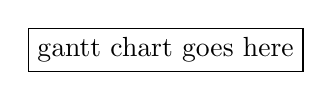
\begin{tikzpicture}
      \node[draw] {gantt chart goes here};
    \end{tikzpicture}
  \caption{Project Gantt Chart}
  \label{fig:gantt}
\end{figure}

Despite best efforts to accurately estimate the amount of time that would be necessary to complete certain tasks, due to lack of experience, some of these were underestimated which meant that, due to time limitations, it was necessary to remove some features from the project scope to ensure that those features which are implemented are completed to a high quality. The Gantt chart served well identifying when tasks were overrunning and could potentially impact the timely delivery of the project as a whole. As the project began falling behind schedule, with tasks such as prototyping the message sending and receiving process taking considerably longer than expected due to the complexitites of the node-imap library, it was decided that file sharing functionality should be excluded from the project scope. This decision was made so that a more essential feature, end-to-end encryption, could be implemented fully and to a high standard, and this was completed on schedule.

Throughout the course of the project, progress was tracked using an online Kanban board on Trello. The benefit of this board is that it was possible to generate a burnup chart, seen in Figure \ref{fig:burnup}, showing the number of work items (cards) completed over time.

Work over the course of the project was relatively consistent, with some time taken for exam revision from December through January. The COVID-19 situation towards the end of the project presented some disruption and uncertainty, however this was primarily during the report writing stage and therefore did not significantly affect progress in terms of development.

\begin{figure}[h!]
  \centering
  \includegraphics[width=\textwidth]{images/burnup.png}
  \caption{Burnup chart showing number of completed work items over time}
  \label{fig:burnup}
\end{figure}

\section{Contributions and Reflections}

% Providing the details of your achievements and contributions including innovation, creativity and novelty (if there is any) as well as a personal reflection on the plan and your experience of the project (a critical appraisal of how the project went).

Overall, I believe that this project has been a success, with high quality, well tested code, culminating in a software product that meets the vast majority of the initial requirements. Writing unit tests often took a considerable amount of time, and this was not factored into the time estimates for task completion, which did lead to changes to the project plan. The project presented a number of challenges, including developing a user interface that supports an excellent user experience as well as working with complex communication protocols such as IMAP. Designing and implementing effective solutions to these has stretched my abilities as a software engineer and enabled me to explore areas that I had not previously had the opportunity to work in.

\section{Future Work}
Despite the significant work that has taken place so far, there is some further work necessary before this software could become a commercially viable product, and there are additional features that could be added. The immediate focus for future work should be to implement the features that were removed from the project scope for various reasons. Following this, further improvements can be made. In addition, the software would benefit from improvements to the current unit and functional testing coverage, to ensure that all further developments are sufficiently regression tested. Some of the key items of work to be completed in the future are; to allow users to send attachments, as was originally planned, which would help to increase adoption of this platform as a new messaging client. In addition; to improve the application's performance, message fetching should be paginated, so that only a subset of a conversation's messages are fetched to begin with (the most recent), and more messages are fetched as the user scrolls back.


\clearpage
\phantomsection
\addcontentsline{toc}{chapter}{Bibliography}
\bibliographystyle{acm}

\mediumlinespacing
\bibliography{bibliography/bibliography}


% appendices come here

\begin{appendices}

% e.g., User Manuals, supporting evidence for claims made in the main part of the dissertation (e.g. a copy of a user evaluation questionnaire), samples of test data, etc. Note that Appendices are optional.

\chapter{Unit Test Coverage Report}
\label{appendix:coverage}
\includegraphics[width=\linewidth]{images/coverage-report.png}

\chapter{User Evaluation Questionnaire}

\end{appendices}


\end{document}